\documentclass[11pt]{scrartcl}
\usepackage[sexy]{ashu}
\usepackage{comment}
\usepackage{ amssymb }
\usepackage{interval}
\usepackage{mathabx,epsfig}

\usetikzlibrary{shapes.geometric}

\usepackage{pst-node,pst-plot}

\usepackage{mathtools}
\newcommand\Set[2]{\{\,#1\mid#2\,\}}
\newcommand\SET[2]{\Set{#1}{\text{#2}}}
\newcommand\setp[1]{\{\,#1\}}
\def\acts{\mathrel{\reflectbox{$\righttoleftarrow$}}}

\begin{document}
\title{Groups Revision Notes IA 2020} % Beginner
\subtitle{Lectured by A. Khukhro}
\date{Michaelmas Term, 2020}
\maketitle

\begin{abstract}
	\sffamily\small
	Life is meaningless

	\medskip

	--- Ashutosh Tripathi
\end{abstract}

\tableofcontents
\newpage


\vspace{1em}
%definitions, itemize, prop, proofs, lemma, theorem

\section{All the Stuff with no Proofs}
\subsection{Groups}
\begin{definitions} [\vocab{Groups}] 
$G$, is defined as a Group  structure if it obeys the following axioms:
\begin{itemize}
    \item (G0) Closure: $\forall x,y \in G$, $xy \in G$
    \item (G1) Associative : $\forall x,y,z \in G$, $ x(yz)=(xy)z\in G$
    \item (G2) Identity : $\exists e \in G$ s.t $\forall x \in G, ex=x=xe$
    \item (G3) Inverse : $\forall x \in G, \exists x^{-1} \in G$ s.t $xx^{-1} = e = x^{-1}x $
\end{itemize}
\end{definitions}

\begin{prop}
For a given group, $G$, the following are true
\begin{enumerate}
    \item $a,b \in G$, $ab=e \implies ba=e$
    \item $a \in G$, $ae=a \implies ea=a$
    \item $a,b \in G$, $ab=e \implies ba=e$
    \item $a,e,e' \in G$, $ae=a \land ae'=a \implies e=e'$
\end{enumerate}
\end{prop}
\subsection{Subgroups}
\begin{definitions}
$H \leq G$ if it satisfies the following axioms
\begin{itemize}
    \item (G0) Closure
    \item (G1) Identity
    \item (G2) Inverse
\end{itemize}
\end{definitions}
\begin{lemma}[\vocab{Subgroup Lemma}]
$H \leq G \iff H\neq \emptyset 
\land \forall a,b \in H, ab^{-1}\in H $ 
\end{lemma}
\begin{definitions}
$\langle X \rangle$ is the notation for the 
\begin{itemize}
    \item Smallest Subgroup of G containing X
    \item $\bigcup_{X \subseteq Y \leq G} Y$
    \item $\Set{\prod_{i=1}^{k}x_{i}^{\alpha_{i}}}{x_{i}\in X, \alpha_{i} \in \setp{\pm 1}, k \in \mathbb{N}^{>0}}$
\end{itemize}
\end{definitions}

\subsection{Homomorphism}

\begin{definitions}[\vocab{Group homomorphism}]
  Let $(G, *)$ and $(H, \times)$ be groups. A function $f:G\rightarrow H$ is a \emph{group homomorphism} iff
  \[
   ( \forall g_1, g_2 \in G)\, \phi(g_1)\times \phi(g_2) = \phi(g_1 * g_2),
  \]
\end{definitions}

\begin{definitions}[\vocab{Group isomorphism}]
  \emph{Isomorphisms} are bijective homomorphisms. Two groups are \emph{isomorphic} if there exists an isomorphism between them. We write $G\cong H$.
\end{definitions}

\begin{definitions}[\vocab{Image of homomorphism}]
  If $\phi:G\rightarrow H$ is a homomorphism, then the \emph{image} of $\phi$ is
  \[
    \im \phi = \phi(G) = \{\phi(g):g\in G\}.
  \]
\end{definitions}

\begin{definitions}[\vocab{Kernel of homomorphism}]
  The \emph{kernel} of $\phi$, written as
  \[
    \ker \phi = \phi^{-1}(\{e_H\}) = \{g\in G:\phi(g)=e_H\}.
  \]
\end{definitions}

\begin{prop}
  Suppose that $\phi: G\rightarrow H$ is a homomorphism. Then
  \begin{enumerate}
    \item Homomorphisms send the identity to the identity, i.e.
      \[
        \phi(e_G) = e_H
      \]
    \item Homomorphisms send inverses to inverses, i.e.
      \[
        \phi(a^{-1}) = \phi(a)^{-1}
      \]
    \item The composite of 2 group homomorphisms is a group homomorphism.
    \item The inverse of an isomorphism is an isomorphism.
  \end{enumerate}
\end{prop}
\begin{prop}
  Both the image and the kernel are subgroups of the respective groups, i.e.\ $\im \phi\leq H$ and $\ker \phi \leq G$.
\end{prop}
\begin{prop}
  For all homomorphisms $f:G\rightarrow H$, $f$ is
  \begin{enumerate}
    \item surjective iff $\im \phi = H$
    \item injective iff $\ker \phi = \{e\}$
  \end{enumerate}
\end{prop}
\subsection{Direct Products}
\begin{definitions}[\vocab{Direct product of groups}]
  Given two groups $(G, \circ)$ and $(H, \bullet)$, we can define a set $G\times H = \{(g, h): g\in G, h\in H\}$ and an operation $(a_1, a_2)*(b_1, b_2) = (a_1\circ b_1, a_2\bullet b_2)$. This forms a group.
\end{definitions}

\begin{theorem}[\vocab{Direct product theorem}]
  Let $H_1, H_2\leq G$. Suppose the following are true:
  \begin{enumerate}
    \item $H_1\cap H_2 = \{e\}$.
    \item $(\forall a_i\in H_i)\, a_1a_2=a_2a_1$.
    \item $(\forall a\in G)(\exists a_i\in H_i)\,a = a_1a_2$. We also write this as $G=H_1H_2$.
  \end{enumerate}
  Then $G\cong H_1\times H_2$.
\end{theorem}

\subsection{Cosets}
\begin{definitions}[\vocab{Cosets}]
  Cosets are fun! They are equivalence classes of an equivalence relation on a group $G$. Basically if $H \leq G$ then the \vocab{left coset} is the set $gH$ where $g\in G$ and $$gH = \Set{g*h}{h\in H}$$\\
  Similarly, we can define $Hg$.
  \\Also $G/H$ is the \vocab{quotient}, the set of all left cosets. Similarly can define $H  \backslash G$ for right cosets.
  \\
  $\vert G/H \vert = [G:H]$, and this is called the \vocab{Index of H in G}
\end{definitions}
\begin{prop}
  If $aH=bH$ then $b^{-1}a \in H$
\end{prop}
\begin{prop}
There is a natural bijection between $gH$ and $H$ and thus $\vert gh \vert = \vert H \vert$
\end{prop}
\begin{theorem}[\vocab{Lagrange's Theorem}]
$$\vert G \vert = [G:H]\vert H \vert$$
\end{theorem}
\begin{prop}
\begin{itemize}
Some easy propositions as a consequence of Lagrange's Theorem
    \item if $\vert G \vert =p $ where $p$ is a prime, then $G$ is a cyclic group
    \item $\ord(g) \mid \vert G \vert$
\end{itemize}
\end{prop}
\begin{definitions}
  $U_{n} = \Set{a \in \mathbb{N}^{>0}}{(a,n)=1}$
\end{definitions}
\begin{theorem}[\vocab{Euler-Fermat}]
$$a^{\phi(n) -1} \equiv 1 \bmod{n} $$
\end{theorem}
\subsection{Normal Groups}
\begin{definitions}
$H\leq G$ then if either of the following holds:
\begin{itemize}
    \item $gH=Hg \forall g\in G$
    \item $gHg^{-1} = H \forall g \in G$
    \item $ghg^{-1} \in H \forall g\in G, \forall h \in H$
\end{itemize}
Then we say $H\mathrel{\unlhd}G$, and we say that \vocab{H is normal in G}
\end{definitions}
\begin{prop}
    New Usual Stuff
    \begin{itemize}
        \item if index of $H$ is $2$ then is normal in $G$
        \item ALl subgroups in abelian groups are abelian
    \end{itemize}
\end{prop}
\subsection{Quotient Groups}
\begin{prop}
Multiplication of cosets naturally is well defined that is $(aH)(bH)=(abH)$
\end{prop}
\begin{definitions}[\vocab{Quotient Groups}]
If $H \mathrel{\unlhd} G$ then the quotient of $H$ in $G$, $G/H$ forms a group under coset multiplication, and is known as the \vocab{Quotient Group}
\end{definitions}
\begin{definitions}
We define the \vocab{Quotient Map} as 
$$\pi : G \rightarrow G/H$$ $$ g \mapsto gH$$
This is a surjective group homomorphism.
\end{definitions}
\subsection{Isomorphism Theorems}
Very Important!
\begin{theorem}[\vocab{The First Isomorphism Theorem}]
If  $\phi: G \to H$ is a group homomorphism then 
$$G/\ker{\phi} \cong \im(\phi)$$
\end{theorem}
\begin{theorem}[\vocab{The Second Isomorphism Theorem}]
If $K \mathrel{\unlhd} G$ and $H \leq G$ then 
$$H/H\cap K \cong HK/K$$
\end{theorem}
\begin{theorem}[\vocab{The Third Isomorphism Theorem}]
If $K \mathrel{\unlhd} G$ and $H \mathrel{\unlhd} G$ and $K \leq H$ then 
$$G/H \cong (G/K)/(H/K)$$
\end{theorem}
\begin{theorem}[\vocab{The Subgroup Correspondence Theorem}]
Let $K \mathrel{\unlhd} G$.\\
There is a bijjection between the subgroups of $G$ containing $K$ and the subgroups of $G/K$. 
\\This bijjection preserves almost anything you can think of, normality, index, containment.
\end{theorem}
\subsection{Cyclic Groups}
\begin{definitions}
$C_{n}$ exiss lol 
\end{definitions}
\begin{prop}
All subgroups of a cyclic group are cyclic
\end{prop}
\begin{prop}
All possible cyclic groups are isomorphic to either $C_{n}$ for some $n$ or $\mathbb{Z}$
\end{prop}
\subsection{Dihedral Groups}
\begin{definitions}
$$D_{2n} = \langle r,s \vert r^n=s^2=e, srs=r^-1\rangle$$
\end{definitions}

\begin{center}
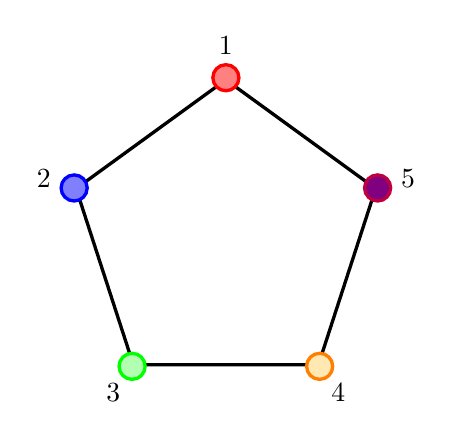
\begin{tikzpicture}[help lines/.style={blue!30,very thin},
 pics/ngon/.style={code={\tikzset{ngon/.cd,#1}
  \node[regular polygon,regular polygon sides=\pgfkeysvalueof{/tikz/ngon/n},
  minimum size=4cm,draw,ngon/border] (\pgfkeysvalueof{/tikz/ngon/name}){};
   \foreach \X in {1,...,\pgfkeysvalueof{/tikz/ngon/n}}
   {\pgfmathsetmacro{\myfillcolor}{{\LstFillCols}[mod(\X-1,5)]}
    \pgfmathsetmacro{\mydrawcolor}{{\LstDrawCols}[mod(\X-1,5)]}
   \path (\pgfkeysvalueof{/tikz/ngon/name}.center) -- (\pgfkeysvalueof{/tikz/ngon/name}.corner \X) 
    node[circle,draw=\mydrawcolor,fill=\myfillcolor,ngon/nodes]{} 
    node[pos=\pgfkeysvalueof{/tikz/ngon/label pos},transform shape=false](\X){\X};
    }
    }},flip about/.style={/utils/exec=\pgfmathsetmacro{\posangle}{%
    -1*iseven(\pgfkeysvalueof{/tikz/ngon/n})*180/\pgfkeysvalueof{/tikz/ngon/n}+%
    (#1-1)*360/\pgfkeysvalueof{/tikz/ngon/n}},
    rotate=\posangle,xscale=-1,rotate=-1*\posangle},
    ngon/.cd,n/.initial=5,border/.style={very thick},nodes/.style={very thick},
    name/.initial={ngon},label pos/.initial=1.2,
    angle of/.code 2 args=\pgfmathsetmacro{#2}{%
    -1*iseven(\pgfkeysvalueof{/tikz/ngon/n})*180/\pgfkeysvalueof{/tikz/ngon/n}+%
    (#1-1)*360/\pgfkeysvalueof{/tikz/ngon/n}}]
 \edef\LstFillCols{"red!50","blue!50","green!30","red!30!yellow!30","red!50!blue"}
 \edef\LstDrawCols{"red","blue","green","orange","purple"}
 \pic{ngon={n=5}};
 \end{tikzpicture}
\end{center}
\subsection{Symmetric Groups}
\begin{definitions}
$S_{n}$ exists lol and so does $A_{n}$
\end{definitions}
\begin{definitions}
$\epsilon(\sigma)$ is the parity of the permutation $\sigma \in S_{n}$. It is equal to $(-1)^{\text{No. of transpositions}}$. Fun fact,it is a surjective group homomorphism from $G$ to $\setp{\pm 1}$
\end{definitions}
\begin{prop}
Disjoint Cycles Commute
\end{prop}
\begin{prop}
All permutations in $S_n$ are expressible as unique product of disjoint cycles
\end{prop}
\begin{prop}
The order of a permutation is the lcm of the orders of all the disjoint cycles
\end{prop}
\begin{prop}
All elements in $S_{n}$ are expressible as a product of transpositions(not necessarily unique)
\end{prop}
\begin{prop}
The above mentioned product of transpositions preserves parity
\end{prop}
\begin{prop}
$A_{n}$ is the kernel of the sign homomorphism
\end{prop}
\begin{prop}
Some Generator Shit:
\begin{itemize}
    \item $S_n = \langle (1i) \rangle$
    \item $S_n = \langle (i,i+1)\rangle$
    \item $S_n = \langle (1 2) (1 2 \ldots n) \rangle$
\end{itemize}
\end{prop}
\begin{prop}
$A_n$ can be generated by 3-cycles for all $n\geq 3$
\end{prop}
\begin{prop}
$A_n$ is simple for $n \geq 5$
\end{prop}
\begin{prop}
The size of conjugacy classes of $S_n$ for $\sigma$ of cycle-type $1^{a_1}2^{a_2}\ldots n^{a_n}$ is 
$$\vert \text{ccl}(\sigma) \vert = \frac{n!}{\prod_{i=1}^{n}(a_{i}! i^{a_i})}$$
\end{prop}
\begin{prop}
Conjugacy Classes in $S_n$ can either split or remain the same to form conjugacy classes for $A_n$, with splitting happening iff $C_{A_n}(\sigma)$ contains an odd permutatation.
\end{prop}
\begin{definitions}
Conjugacy Classes may split if $\sigma$'s disjoint cycle representation has distinct odd-length cycles.
\end{definitions}
\begin{definitions}
A subgroup $H \leq S_n$ has either 0 or exactly half the number of odd permutations
\end{definitions}

\subsection{Groups of Small Order}
\begin{definitions}[\vocab{Quarternion}]
$$Q_8 = \langle -1,i,j,k \vert (-1)^2=1, i^2=j^2=k^2=ijk=-1\rangle$$
\end{definitions}
\begin{prop}
Well let's just list some stuff, besides the obvious for primes
\begin{itemize}
    \item $4$ : $C_2 \times C_2 $, $C_4$
    \item $6$ : $C_6$, $S_3$
    \item $8$ : $C_2 \times C_2 \times C_2$, $C_4 \times C_2$, $D_8$, $Q_8$, $C_8$
\end{itemize}
\end{prop}

\subsection{Group Actions-an Intro}
\begin{definitions}[\vocab{Group Action}]
Group actions are binary operations of a group $G$ on a set $X$ defined from $G \times X \to X$ such that 
\begin{itemize}
    \item Closure : $g(x) \in X \forall x \in X, \forall g \in G$
    \item Associativity : $g(g'(x))=gg'(x) \forall g,g' \in G, x \in X$
    \item Identity : $e(x)=x$
\end{itemize}
\end{definitions}
\begin{definitions}[\vocab{Orbits}]
$$\text{orb}(x)=\Set{g(x)}{g \in G}$$
If $orb(x)=X \forall x \in X$ then the group action is transitive
\end{definitions}
\begin{definitions}[\vocab{Stabilizer}]
$$\text{stab}(x) = \Set{g\in G}{g(x)=x}$$
\end{definitions}
\begin{definitions}[\vocab{Kernel}]
$$\bigcap_{x \in X} \text{stab}(X)$$
If kernel of a group action is trivial, then the group action is faithful
\end{definitions}
\begin{prop}
Group action is a homomorphism, that is if $G \acts X \iff \exists \rho \text{ s.t } \rho : G \rightarrow X$
\end{prop}
\begin{theorem}[\vocab{Cayley}]
$G \cong M \leq \text{Sym}(G)$
\end{theorem}
\begin{prop}
This is easy to see:
\begin{itemize}
    \item $\text{stab}(x) \leq G $
    \item orb($x$) partitions $X$
\end{itemize}
\end{prop}
\begin{theorem}[\vocab{Orbit-Stabilizer}]
Assume $G \acts X$ \\
$\vert G \vert = \vert \text{orb}(x) \vert \vert \text{stab}(x) \vert \forall x\in X$
\end{theorem}
\begin{theorem}[\vocab{Cauchy}]
If $p \mid \vert G \vert \implies \exists g \in G \text{ s.t } \ord(g) = p$
\end{theorem}

\subsection{Conjugation Action}
\begin{definitions}[\vocab{Conjugation Action}]
$G \acts G$ such that $g(\alpha)=g\alpha g^-1$
\end{definitions}
\begin{definitions}[\vocab{Centralizer}]
The stabilizer of $g$ for conjugation group action is the \vocab{Centralizer}, $C_{G}(g)$
\end{definitions}
\begin{definitions}[\vocab{Conjugacy Classes}]
The orbit of the conjugation group action for $g$,$\text{ccl}(g)$
\end{definitions}
\begin{definitions}[\vocab{Center}]
The kernel of the conjugation action, $Z(G)$
\end{definitions}
\begin{prop}
Conjugation preserves order, thus conjugacy classes consist of elements that have the same order
\end{prop}
\begin{prop}
Normal Subgroups of $G$ are unions of conjugacy classes
\end{prop}
\begin{prop}
$Z(G) \mathrel{\unlhd} G$
\end{prop}
\begin{prop}
$Z(G)$ consists of elements with singleton conjugacy classes
\end{prop}
\begin{definitions}[\vocab{Normalizer}]
	For any subgroup $H$ of $G$ the \vocab{normalizer} of $H$ is defined as
	\[ N_G(H) \defeq \left\{ g \in G \mid gHg\inv = H \right\}. \]
	In other words, it is the stabilizer of $H$ under the conjugation action.
\end{definitions}
\subsection{Sylow's Theorems}
\begin{theorem}[The Sylow theorems]
	Let $G$ be a group of order $p^n m$,
	where $\gcd(p,m)=1$ and $p$ is a prime.
	A \vocab{Sylow $p$-subgroup} is a subgroup of order $p^n$.
	Let $n_p$ be the number of Sylow $p$-subgroups of $G$.
	Then
	\begin{enumerate}[(a)]
		\ii $n_p \equiv 1 \pmod p$. In particular, $n_p \neq 0$ and
		a Sylow $p$-subgroup exists.
		\ii $n_p$ divides $m$.
		\ii Any two Sylow $p$-subgroups are conjugate subgroups (hence isomorphic).
	\end{enumerate}
\end{theorem}
\begin{prop}
These are direct results of sylow's theorems
\begin{itemize}
	\ii A Sylow $p$-subgroup is normal if and only if $n_p = 1$.
	\ii Any group $G$ of order $pq$, where $p < q$ are primes,
	must have $n_q = 1$, since $n_q \equiv 1 \pmod q$ yet $n_q \mid p$.
	Thus $G$ has a normal subgroup of order $q$.
	\ii Since any abelian group has all subgroups normal,
	it follows that any abelian group has exactly one Sylow $p$-subgroup
	for every $p$ dividing its order.
	\ii If $p \neq q$, the intersection of a Sylow $p$-subgroup and a Sylow $q$-subgroup is just $\{1_G\}$.
	That's because the intersection of any two subgroups is also a subgroup,
	and Lagrange's theorem tells us that its order must divide both a power of $p$
	and a power of $q$; this can only happen if the subgroup is trivial.
\end{itemize}
\end{prop}
\subsection{Mobius Groups}
\begin{definitions}[\vocab{Mobius Maps}]
It is a map $f: \hat{\mathbb{C}} \rightarrow \hat{\mathbb{C}} $ such that 
\[
  f(z) =
  \begin{cases}
                                 \frac{a}{c} & \text{ if $z=\infty$} \\
  \infty & \text{if $z=\frac{-d}{c}$} \\
                      \frac{az+b}{cz+d} & \text{otherwise} 
  \end{cases}
\]
\end{definitions}
\begin{definitions}[\vocab{Mobius Groups}]
The set of mobius maps $\mathcal{M}$ under composition forms a non-abelian group
\end{definitions}
\begin{prop}
Mobius Group Acts on the extended complex numbers set $\hat{\mathbb{C}}$
\end{prop}
\begin{prop}
Mobius Group is generated by 
\begin{itemize}
    \item Dilation/Rotation
    \item Translation
    \item Inversion
\end{itemize}
\end{prop}
\begin{prop}
A mobius map with $\geq 3$ fixed points is identity map.
\end{prop}
\begin{prop}
If two mobius maps $f$ and $g$ agree at atleast 3 points then $f=g$
\end{prop}
\begin{prop}
A Mobius map can be completely determined by knowing what happens to 3 points. If $f$ is a mobius map such that $(z_1,z_2,z_3) \mapsto (0,1 \infty)$ then 
$$f(z)=\frac{(z_2-z_3)(z-z_1}{(z_2-z_1)(z-z_3)}$$
\end{prop}
\begin{prop}
Conjugation of mobius maps preserves order and also if $f$ has fixed point $g$ then the fixed point of $hfh^-1$ is $h(g)$
\end{prop}
\begin{prop}
A non-identity mobius map has either 1 or 2 fixed points and depending on the number of fixed points:
\begin{itemize}
    \item 1 $\implies$ Conjugate to $z+1$
    \item 2 $\implies$ Conjugate to $\alpha z$
\end{itemize}
\end{prop}
\begin{definitions}[\vocab{Circles}]
$Az\Bar{z} + B\Bar{z} + \Bar{B}z + C = 0$
\end{definitions}
\begin{prop}
Mobius Maps takes a circle to another circle
\end{prop}
\begin{definitions}[\vocab{Cross Ratio}]
If $f$ is a mobius map such that $(z_1,z_2,z_3) \mapsto (0,1,\infty)$ for distinct $z_1,z_2,z_3,z_4 \in \hat{\mathbb{C}}$ then $$[z_1,z_2,z_3,z_4] = f(z_4)$$
\end{definitions}
\begin{prop}
$$[f(z_1),f(z_2),f(z_3),f(z_4)] = [z_1,z_2,z_3,z_4]$$
\end{prop}
\begin{prop}
$$z_1,z_2,z_3,z_4 \text{ lie on the same circle }\iff [z_1,z_2,z_3,z_4] \in \mathbb{R}$$
\end{prop}
\subsection{Matrix Groups}
\begin{definitions}
The set of all $n x n$ matrices over field $\mathbb{F}$ form a group $M_{nxn}(\mathbb{F})$
\end{definitions}
\begin{definitions}[\vocab{General Linear Group}]
The set of all $nxn$ invertible matrices over field $\mathbb{F}$ such that the determinant is 1 is the \vocab{General Linear Group}. $GL_n(\mathbb{F})$ 
\end{definitions}
\begin{definitions}[\vocab{Special Linear Group}]
The set of all $nxn$ invertible matrices over field $\mathbb{F}$ such that the determinant is 1 is the \vocab{Special Linear Group}. $SL_n(\mathbb{F})$
\end{definitions}
\begin{prop}
$det : GL_n(\mathbb{F}) \rightarrow \mathbb{F}^{*} $ has kernel $SL_n(\mathbb{F})$
\end{prop}
\begin{definitions}[\vocab{Orthogonal Group}]
The set of all $nxn$ Real Orthogonal Matrices $A^T A =I$
\end{definitions}
\begin{definitions}[\vocab{Special Orthogonal Group}]
The set of all $nxn$ Real Orthogonal Matrices $A^T A =I$ and $\text{det}(A)=1$
\end{definitions}
\begin{definitions}[\vocab{Unitary Group}]
The set of all $nxn$ Unitary Matrices.
\end{definitions}
\begin{definitions}[\vocab{Special Unitary Group}]
The set of all $nxn$ Unitary Matrices with determinant 1
\end{definitions}
\begin{prop}
The Mobius group can also be seen as matrix shit :
$$\theta : SL_{2} \to \mathcal{M}$$
$\theta$ is a surjective homorphism with kernel $\setp{\pm I}$ and the quotient group $SL_{2}/\setp{\pm I} \cong PSL_2$, the projective special linear group. 
\end{prop}
\begin{prop}
The Matrix Groups can act on their respective Fields, kinda sick.
\end{prop}
\begin{prop}
Change of Basis is basically if $A$ is a matrix that represents a particular transformation wrt basis $\setp{e_i}$, and $A'$ represents the same transformation wrt basis $\setp{f_a}$ then there exists a matrix $P$ called the change of basis matrix such that $f_a=P_ia e_i$ (summation convention applies) such that $A'=P^{-1}AP$
\end{prop}
\begin{prop}
Change of Basis is basically a conjugation action. Jordan Normal Form is also a conjugation action
\end{prop}
\begin{prop}
This is recap stuff from V+M about orthogonal matrices 
\begin{itemize}
    \item Orthogonal Matrices' columns are orthonormal to each other thus form an orthonormal basis 
    \item Orthogonal Matrices preserve length and angles
    \item Reflection matrix is a type of orthogonal matrix
    \item $P^{-1}R_aP = R_{Pa}$
    \item Determinant of $R_a$ is -1 always
    \item if working in $\mathbb{R}^{3}$ then if an orthogonal matrix has determinant 1 then 1 is an eigenvalue
\end{itemize}
\end{prop}
\begin{prop}
$SO_2$ consists of rotation matrices, of the form $\begin{pmatrix}
  \cos(\theta) & -\sin(\theta)\\ 
  \sin(\theta) & \cos(\theta)
\end{pmatrix}$
\end{prop}
\begin{prop}
$O_2 / SO_2$ consists of only reflections
\end{prop}
\begin{prop}
Every element in $O_2$ can be generated by, at max, product of 2 reflection matrices
\end{prop}
\begin{prop}
$SO_3$ consists of matrices of the form $\begin{pmatrix}
 1 & 0 & 0\\
 0 & \cos(\theta) & -\sin(\theta)\\ 
 0 & \sin(\theta) & \cos(\theta)
\end{pmatrix}$
\end{prop}
\begin{prop}
$O_3/SO_3$ consists of only reflections
\end{prop}
\begin{prop}
Every element in $O_3$ can be represented by a product of maximum 3 reflection matrices
\end{prop}
\subsection{Symmetries of Platonic Solids}
\begin{prop}
Platonic Solids kinda cool, and all are subgroups of $O_3$
\begin{itemize}
    \item Tetrahedron symmetries are the group $A_4$ 
    \item Cube symmetries are the group $S_4$. Since Octhedral is a dual of cubes, implies the orientation preserving symmetries are $S_4$ and all symmetries are $S_4 \times C_2$ and this is known as the  \vocab{Octahedral Group}
    \item Dodecaheron Symmetries are the group $A_5$. Since icosahedron is a dual of dodacehdron implies theorientation preserving symmetries are $A_5$ andall symmetries are $A_5 \times C_2$ and this is known as the \vocab{Icosahedral Group} 
\end{itemize}

\end{prop}
%------------------------------------------------------


\end{document}
